\section{Results}
Once the actual experiments began, several changes had to be made to the configurations of the runs, because the generated strategies rapidly overfitted to the train data.

First of all, a different trace file was chosen for the subsequent runs. The chosen trace file was the 'crafty\_mem.trace'. The first 20000 requests were used as the train dataset, and the subsequent 200000 requests were used as the test dataset. The train dataset contained 1181 unique page requests, and the test dataset contained 2646 unique page requests. This trace file was chosen because it contained fewer unique page requests and more repetition that the 'swim.trace' file, so it seemed like a good fit for evolving cache replacement policies.

Secondly, some parameters of the runs were changes. Population size was increased to 200, and each run consisted of 200 generations. These changes were implemented to cultivate the exploration of the search space. Mutation rate was decreased from 20\% to 5\%, as the rate of 20\% seemed very disruptive.

Another problem that emerged was that the strategies did not evolve at all, since the strategy in which they do nothing and the page from the frame at index 0 is always removed worked relatively well. This was the default strategy since the index of the frame from which the page would be removed was a program variable that was initialized to 0. There was a similar problem where the evolution would find clearly nonsensical and unusable strategies. Two of the most popular strategies that fall into this category were the strategy to choose the frame that corresponds to the time variable and the strategy to choose the frame at the index which is equal to the index of the requested page. A solution to this problem was checking if the strategy doesn't set the frame variable, or if it sets it to the time variable or the requested page index variable, and if some of these cases were true, the strategy would be penalized with the fitness of zero.

Finally, while loops were removed from the grammar for these runs. The reason behind this decision was that the strategies found it very hard to use them in a smart way (like the CLOCK strategy use a while loop), and they drastically increased the simulation times, to the point where it would be impossible to run all the simulations in an acceptable timespan. The most common problem with while loops was that the strategies would leave their bodies empty or fill them with nonsensical instructions, and this would be calculated for every frame (since the maximum number of iterations is equal to frame count), for every page request in the data set, for every strategy that used while loops, for every generation, for every run of the experiment.

Four different experiments were run, each with a different cache size. For each experiment, a bar plot will be included, showing the hit counts of the strategies OPT, FIFO, CLOCK, LRU, LFU, as well as three chosen strategies generated by the grammatical evolution, and they will be marked as GE1, GE2, GE3. Each experiment was run 10 times, and each run had population of 200, so for every experiment, 2000 strategies from the last generations were tested using the test data. There was a lot of repetition in the generated strategies and the hit counts, so the values for the strategies GE1, GE2 and GE3 were chosen as the three best unique scored hit counts.

\subsection{Experiment 1: frame count 100}

\begin{figure}[H]
	\centering
	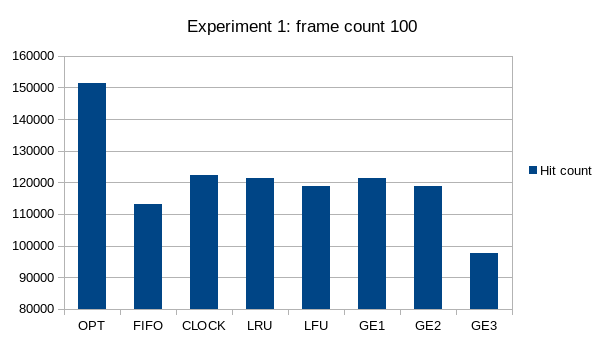
\includegraphics[scale=0.55]{bar_plot_06.png}
	\caption{Results of experiment with the frame count set to 100}
\end{figure}

\subsection{Experiment 2: frame count 200}

\begin{figure}[H]
	\centering
	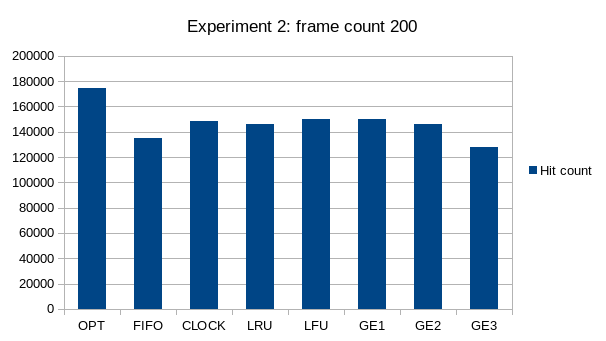
\includegraphics[scale=0.55]{bar_plot_07.png}
	\caption{Results of experiment with the frame count set to 200}
\end{figure}

\subsection{Experiment 3: frame count 300}

\begin{figure}[H]
	\centering
	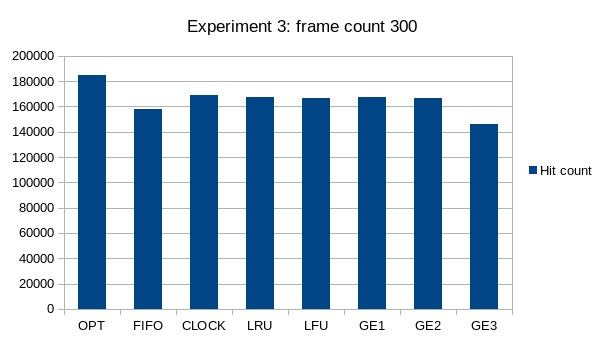
\includegraphics[scale=0.55]{bar_plot_08.png}
	\caption{Results of experiment with the frame count set to 300}
\end{figure}

\subsection{Experiment 4: frame count 500}

\begin{figure}[H]
	\centering
	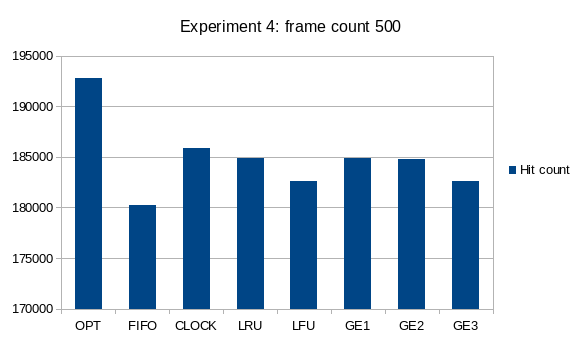
\includegraphics[scale=0.55]{bar_plot_09.png}
	\caption{Results of experiment with the frame count set to 500}
\end{figure}

\subsection{Results analysis}
During all the runs, the best strategies that the evolutionary search managed to find were equivalent to one of the heuristic strategies, namely the LRU and LFU strategies. Unfortunately, the generated strategies never managed to learn how to use the info arrays or develop any complex behaviour, so it seems that expecting the genetic algorithm to develop and learn such behaviours may have been too ambitious. Nevertheless, the algorithm always converged and resulted in strategies that can compare to classic heuristic approaches. 

One interesing property that the computer programs written by humans usually possess, and the computer programs generated by genetic programming techniques usually don't possess, is the property of parsimony. If something is parsimonius, it is as simple as it can be while performing its function, and this principle is often called Occam's razor. Like the genome of living beings, programs generated by genetic programming are rarely minimal structures for performing their tasks, instead, they are packed with unused substructures that usually reflect their evolutionary history, not their functionality \citep{koza1992geneticprogramming}. 

Programs generated by genetic programming usually contain parts which aren't used for anything, or expressions which are much more complicated than they need to be. As humans, we prefer computer programs which are easy to read and not more complex than they need to be, so if genetic programming is used to generate programs for a certain task, it would be a good idea to have a human manually inspect the generated programs, or to have them inspected by a code analysis software.

\subsection{Examples of generated strategies}
The following strategy is a good example of non-parsimonious code. This strategy is equivalent to the LFU strategy, but it sets the $accessed$ info array, even though it never uses that information. The strategy would be functionally identical if we were to remove that unnecessary code.
\noindent
\begin{algorithmic}
\State $ frame=page\_access\_count\_min();$
\State $ set\_accessed(num1!=num3,frame);$
\end{algorithmic}

\medskip

Another interesting example is the following generated strategy. This strategy is also equivalent to the LFU strategy, even though the $num3$ variable is being added to the $frame$ variable, because the $num3$ variable is initialized to zero and never changed, so the strategy would be functionally the same if there was no addition.
\noindent
\begin{algorithmic}
\State $ frame=page\_access\_count\_min()+num3;$
\end{algorithmic}

\newpage

The next strategy is really interesting. It is almost identical to to the LRU strategy, except it uses the information about the least recently used frame that was accurate one request ago, and now it's slightly outdated. This strategy was 0.03\% worse than the LRU strategy during the experiments with the frame count of 500.
\noindent
\begin{algorithmic}
\State $ frame=num2;$
\State $ num2=last\_accessed\_min();$
\end{algorithmic}

\medskip

The generated strategies were sometimes really long and unreadable. An example of this is the following strategy.
\noindent
\begin{algorithmic}
\State $ write(1,page\_access\_count\_min(),num3<=num1);$
\State $ if(find\_max(2)*page\_access\_count\_min()<time)$
\State $\{if(num1<=frame==time)\{\}\}else\{\} set\_accessed(num1,frame);$ \State $if(frame)
\{write(1,frame,page\_access\_count\_min());\}$
\State $else\{set\_accessed(num3,find_max(2) * page\_access\_count\_min()<time>=frame);num1=frame==time;\}$
\end{algorithmic}

\medskip

The next strategy is the final strategy we're going to discuss, and it's interesting for two reasons. First, we can notice that it has an expression which looks like $x - false - y$, which is functionally equivalent to $x - y$. Secondly, we can notice that the whole expression is actually a comparison using the $>$ operator. The whole expression can be evaluated either to 1 if it's true, or to 0 if it's false, so this strategy can remove pages only from its first two frames.
\noindent
\begin{algorithmic}
\State $ frame=division(frame<=page\_access\_count\_min()-false-num1>=num2==last\_accessed\_max()-frame>frame>=frame,time)>page\_access\_count\_min();$\end{algorithmic}
